\documentclass[linenumbers]{aastex631}


\newcommand{\vdag}{(v)^\dagger}
\newcommand\aastex{AAS\TeX}
\newcommand\latex{La\TeX}

\nolinenumbers


\begin{document}

\title{Mass Transfer from Tidal Forces in the MW-M31 Merger}


\author{Aidan J. Nakhleh}
\affiliation{University of Arizona}

\section{Introduction} \label{sec:intro}

When galaxies interact with each other gravitationally, dynamical effects alter their structures. Specifically, tidal forces that are brief but very strong distort the outer parts of the interacting disk-shaped galaxies. These distortions take on different forms, and have differing effects on the resulting galactic evolution after the interaction. Some of these effects include satellite formation, star formation and quenching, mass transfer between galaxies, and ejection of material from the entire system.

    These dynamical effects impact kinetic properties of the galaxy, the total mass of the galaxy, and the distribution of different matter within and around the galaxy. These changes can influence the rate of star formation, mass, density, and luminosity profiles, and even the existence of satellites, all influencing the evolutionary track and categorization of the galaxies affected during the merger. 

    The two main characteristics formed during gravitational interaction are galactic tails and bridges. Both of these are formed from tidal forces acting on the outer parts of galactic disks when they interact with each other (\cite{toomre1972galactic}). If conditions are right, some disk material can gain a large velocity kick, and begins to move away from its host galaxy in a thin tail. If there is enough of a kick, the tail can become unbound and escape the system, otherwise it returns back to the system and can connect with either of the two galaxies, or form a separate satellite. Another distortion is the tidal bridge, which features outer disk material of the two galaxies forming a tight line from galactic center to galactic center. This bridge allows for very direct, albeit brief, mass transfer. If the bridge is rich in gas, and it falls to the center of the companion galaxy, a process called AGN feedback can occur, which influences galactic growth and the process of quenching (\cite{ji2014lifetime}). Conversely, in the process of tail creation the velocity kick can induce shock waves which can trigger star formation as well (\cite{barnes2004shock}). 

    \begin{figure}[h!]
        \centering
        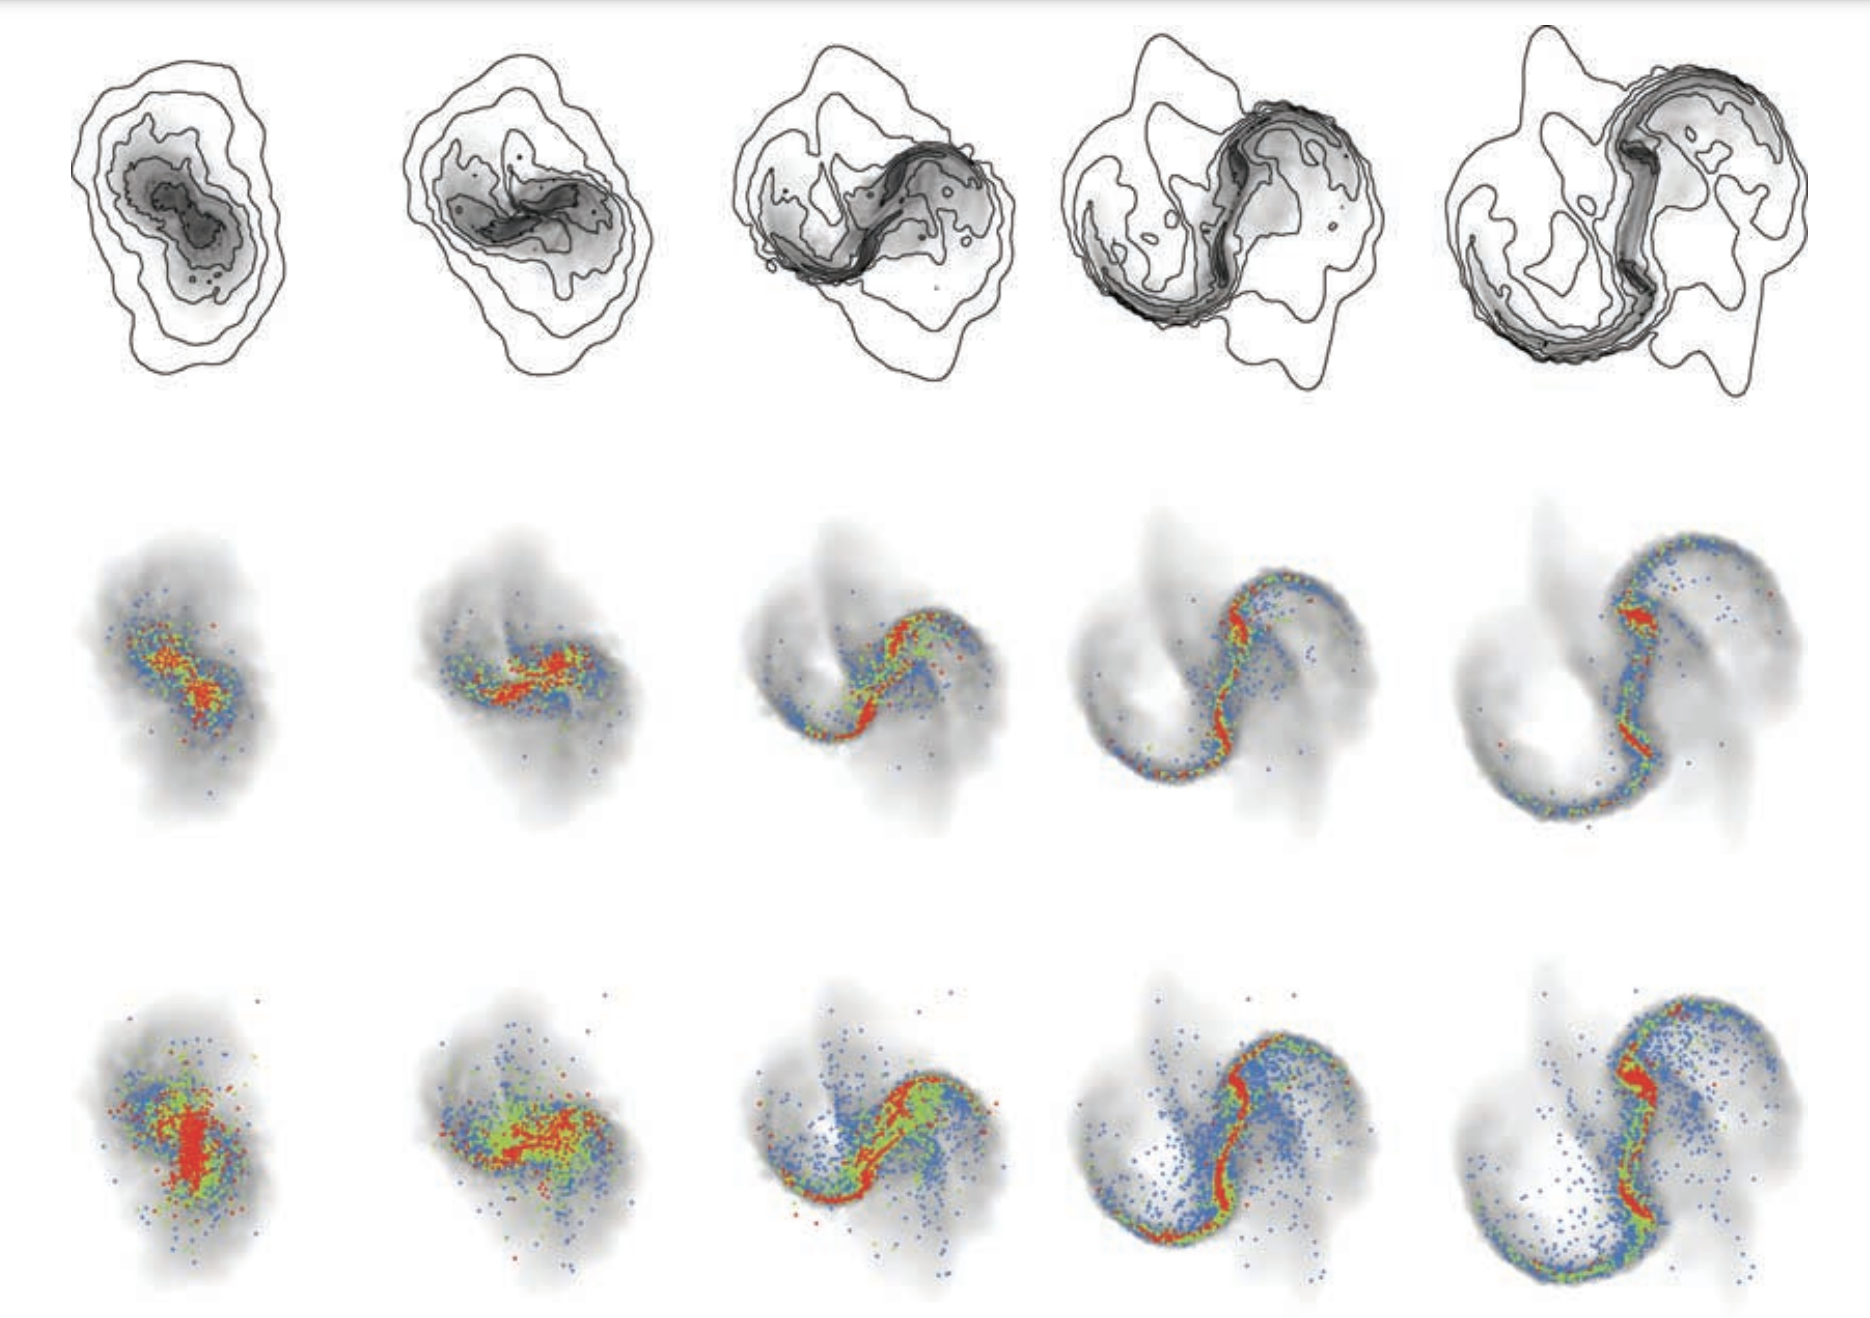
\includegraphics[scale = 0.3]{galaxy_fig.png}
        \caption{From \cite{barnes2004shock}, detailing simulation of the Mice Galaxies (NGC 4676) and their dynamical evolution. This figure tracks star forming regions at different time units using a color coded tagging method. The top row involves contours of gas densities, the second and third rows detail star formation regions through points as they evolve over time. I wish to tag my particles of interest similarly, but instead particles that are part of the tidal bridges and tails in MW and M31. }
        \label{fig:evolution}
    \end{figure}

    The theories of shock induced star formation and density dependent star formation are coupled together by broader dynamics induced during galaxy encounters, so while shock induced star formation does seem to exist, it is not unified yet, and cannot predict star formation properly before the interaction occurs (\cite{barnes2004shock}). Additionally, many of these mergers have been modelled using N-body simulations with gravity as the only contributing force. To obtain a more complete model of how these tails affect star formation, AGN feedback, and gas physics, these N body simulations will need to include hydrodynamics and smaller scale interactions at the sub-grid level (\cite{privon2013dynamical}), and the computational costs need to be reduced for the calculations to be feasible.


\section{Proposal} \label{sec:style}

I will be exploring the mass transfer between the Milky Way and Andromeda galaxies when they interact. Specifically, I will be seeing how much mass flows from one to another, and where that mass flows to. It could move towards the center of either galaxy through a tidal bridge, or outwards in a tidal tail. This flow can suggest to us whether AGN feedback is a significant feature, and how star formation may begin or end. 

To approach this question I will need to create visualization software to inspect the galaxies at different times. As demonstrated by \cite{toomre1972galactic}, the tidal tails and bridges are easily visible as they begin to form. We've done similar work when we identified the substructure of the M31 disk in Lab 7. What's needed here is to tag and track particles within these tidal bridges and tails to see how they evolve with time. As a start, I can find the snap number when the tails and bridges are most clear. I can then select all of the particles in that specified region, and tag them. What I will then need is new code to trace those same particles back and forth through through different snap numbers. Going forward in time and looking at the tracked particles in one galaxy now inside the other galaxy and summing their masses gives an estimate of the mass transfer taking place. This ability to go back and forward in time and tagged particles also suggests where the flow is directed, and how fast the particles are moving. 

Another option is to calculate the potential energy of each particle relative to its host galaxy using the $\Phi$ function, and then compare that to the kinetic energy of the particle, and see which galaxy the particle is bound to, if either of them. Depending on the answer they can be tagged, and traced similarly. Either way, this method of tracking will let me probe how much mass transfer/mass ejection occurs, and where the mass flows to within each galaxy. As a check, I can also find the integrated mass of each galaxy by summing over the masses of the particles, and comparing that answer over time to see how it changes, i.e. how much it gains or loses at different snap numbers. This could be done using the MassEnclosed function developed earlier.

    \begin{figure}[h!]
        \centering
        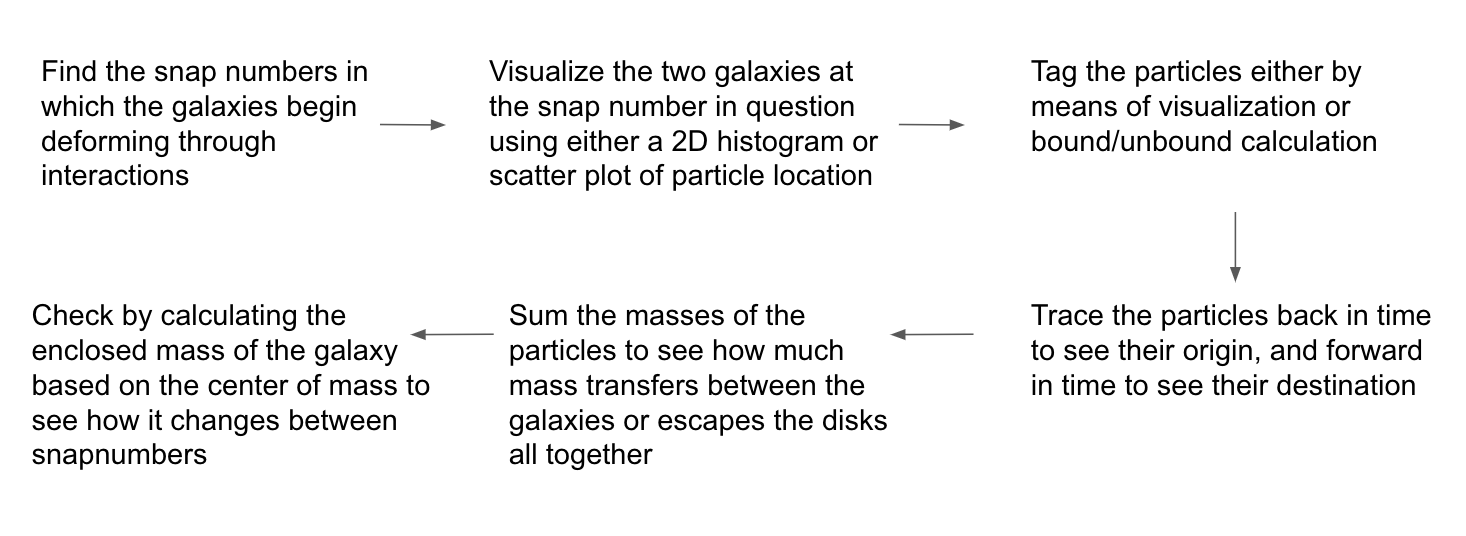
\includegraphics[scale = 0.4]{methodology.png}
        \caption{Flowchart designating how my research will progress step by step with broad methods for each step.}
        \label{fig:methodology}
    \end{figure}

I believe that a relatively small amount of mass transfer will occur on the scale of the galaxy mass, but potentially large on the scale of stellar mass. I believe this will be the case because \cite{toomre1972galactic} mentions, galactic bridges are very transient phenomena so there is not a lot of time for mass transfer to take place. These galaxies will also swing by each other multiple times before merging, which means there will be several opportunities for mass transfer to occur, which means mass can oscillate back and forth between the galaxies several times, reducing the net mass transfer. That being said there can and probably will still be a profound effect on the mass close to the center of each galaxy. Additionally the formation of possible satellites and/or tidal tails that are stretched far away from the disks of the galaxies after they interact and eventually merge may be formed as well, according to existing theories of satellite formation. 

\bibliography{sample631}{}
\bibliographystyle{aasjournal}

\end{document}

